\newpage
\chapter*{Research Question 3}
\addcontentsline{toc}{chapter}{Research Question 3}
% Chapter for each research question
% how we validated it and proved it worked

\textit{What \gls{SDR} tools, processes and or algorithms need to be developed to identify instances of the three main \gls{DAM} emission types detailed in Table. \ref{tab:dam_emissions}?}

\begin{itemize}
	\item Can existing tools and signal processing techniques be employed to find \gls{DAM} emissions?
	\item What is required from an algorithm which might identify \gls{DAM} emissions within an \gls{IQ} signal?
\end{itemize}

\section*{Capturing DAM Emissions with the RTL2832 DAB SDR}
\addcontentsline{toc}{section}{Capturing DAM Emissions with the RTL2832 DAB SDR}

The Radio Jupiter Pro tool was used to choose a date which was optimal for capturing \gls{DAM} emissions. The Figure: \ref{fig:gqrx_spectrogram_01}, was generated by taking a screen capture of the GQRX tool while connected to the HackRF \gls{SDR} transceiver. The data was recorded at a bandwidth of 3MHz for an estimated 2 minutes. The multiple short wide bandwidth bursts are possibly instances of Jovian storm L-Bursts. This spectrogram is a very narrow window considering the capabilities of the HackRF device which has a maximum bandwidth of 20MHz. Unfortunately the HackRF is limited by the USB transfer speeds of the host computer, and the observations were recorded on a machine with USB 2.0, which prevented data being collected at larger bandwidths. Being limited to 2 minutes per screen capture is potentially of little value in hunting for \gls{DAM} emissions, as Jovian storms may occur over several hours. Ideally a spectrogram plot generated from 24 hours worth of data is required.

Due to its recent release there is currently no tools available which are capable of interfacing with the HackRF \gls{SDR} transceiver in order to generate a spectrogram plot from saved data. This speed limitation along with the lack of tooling, raised the possibility of using other devices. The first option being the RTL line of DAB TV receivers which are known to make reasonable \gls{SDR} receivers, and have a wide selection of tooling already developed. The \textit{rtl\_power} utility is shipped with the firmware required to operate the \gls{SDR} receiver and is capable of collecting power data over long periods of time with the view to generate spectrogram plots at a later point. One such tool is the \textit{heatmap.py} utility which is designed to take the output from rtl\_power and produce large bandwidth long period spectrogram plots \citep{keen-15}. This was ideal for the purpose of hunting for \gls{DAM} emissions.

The RTL based receivers have a similar operating range to the HackRF and align somewhat closely with the requirements to pick up \gls{DAM} emissions from Jupiter \citep{hamradioscience-12}. Table: \ref{tab:rtl_vs_hackrf} lists the operating ranges of both the HackRF and also the RTL DAB receiver. The RTL DAB receiver operates at 24MHz at the lower end of its operational range. This is still well within the 7MHz - 40MHz range of Jovian \gls{DAM} emissions, but it is just outside the ideal range recommended by NASA's Radio Jove documentation of 20.1 MHz \citep{nasa12}. The RTL device has a narrow maximum bandwidth of 2MHz, however this is potentially not such an issue, as rtl\_power is designed to quickly retune the receiver and take a power reading to enable the sampling of large bandwidths. The retuning of the RTL receiver in order to take a power sample is not instant. It can take several seconds to take a single reading for a large bandwidth so this should be taken into account \citep{keen-15}.

%
\begin{table}
	\centering
	\begin{tabular}{p{4cm} l}
		\toprule
		Device & Operating Range\\ \midrule
		HackRf & 1MHz - 6GHz \\
		RTL2832U/R820T & 24MHZ - 1850MHz \\
		SDRT & 7MHz - 40MHz \\
		\bottomrule
	\end{tabular}
	\caption{RTL vs HackRF and SDRT Requirements}
	\label{tab:rtl_vs_hackrf}
\end{table}
%

\subsection*{Methodology}
The following methodology was followed during this experiment:

\begin{enumerate}
	\item RTL2832U/R820T Dongle connected to the 21MHz Dual Dipole Array
	\item rtl\_power was left running for 24 hours at a time recording data
	\item A spectrogram was generated using the heatmap.py utility from data collected in the previous 24 hours
\end{enumerate}

The plots shown in Figures: \ref{fig:rtl_power_spectrogram} and Figures: \ref{fig:rtl_power_spectrogram_dam} show possible instances of \gls{DAM} emissions captured using the RTL receiver over extended recording sessions of 24 hours. In Figures: \ref{fig:rtl_power_spectrogram_02} and  \ref{fig:rtl_power_spectrogram_03}, it is possible to see the interference from amateur radio signals while Figures: \ref{fig:rtl_power_spectrogram_dam} also show the extra noise and interference generated by the Sun when it is above the horizon and crosses into the antenna beam. Using both the rtl\_power and heatmap.py utilities, it seems feasible to capture \gls{DAM} emissions on a spectrogram.

%
\begin{figure}
	\centering
	\begin{subfigure}[t]{9cm}
		\centering
		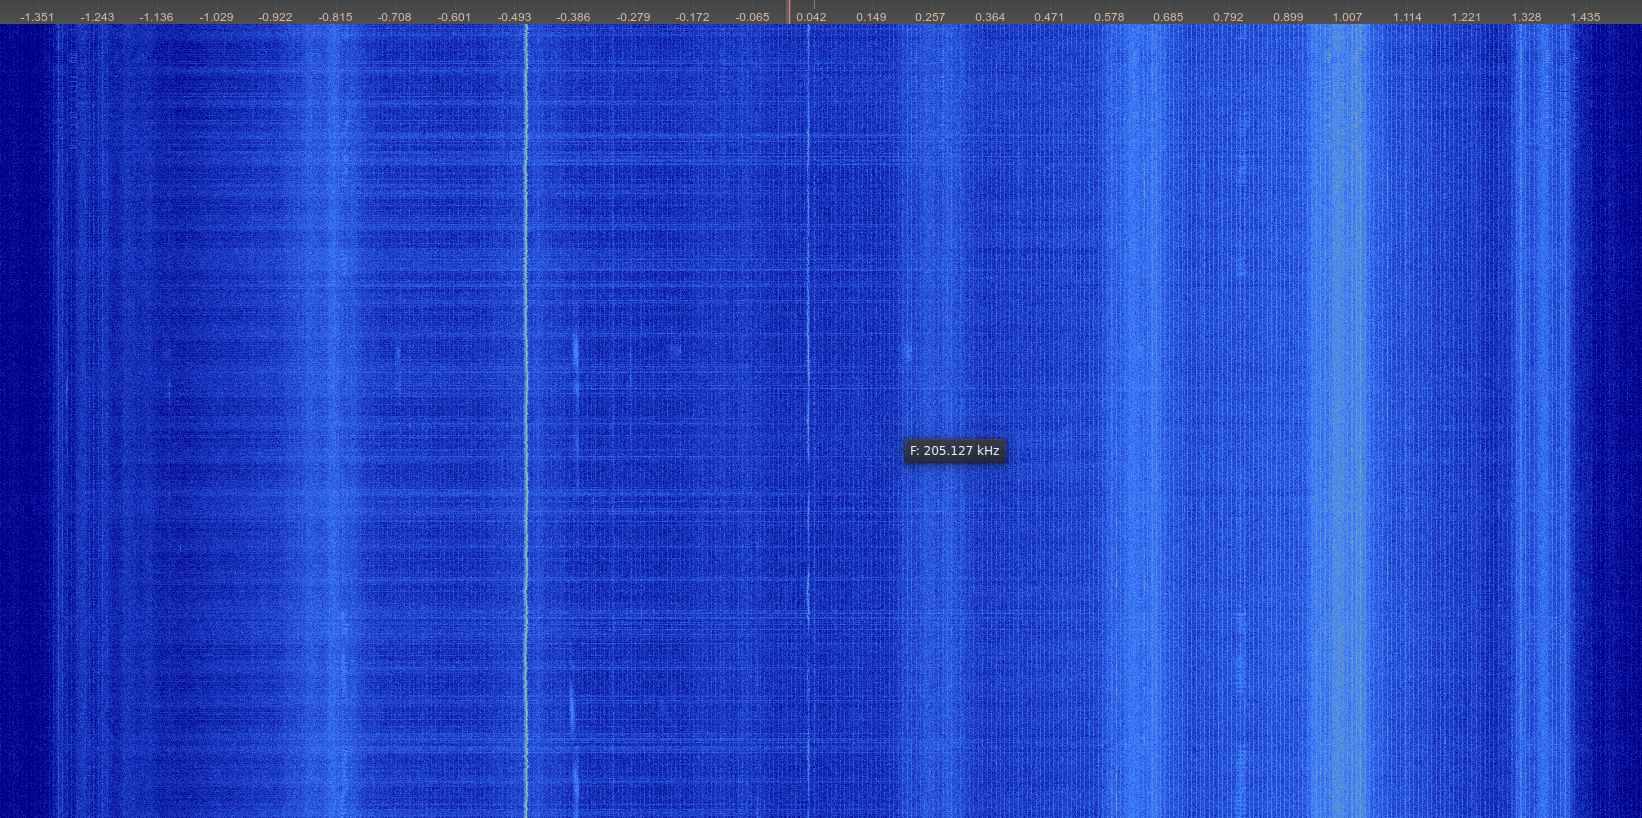
\includegraphics[width=9cm]{images/51}
		\caption{19MHz - 21MHz Spectrogram Built from GQRX 15th April 2015}
		\label{fig:gqrx_spectrogram_01} 
	\end{subfigure}
	\quad
	\begin{subfigure}[t]{5cm}
		\centering
		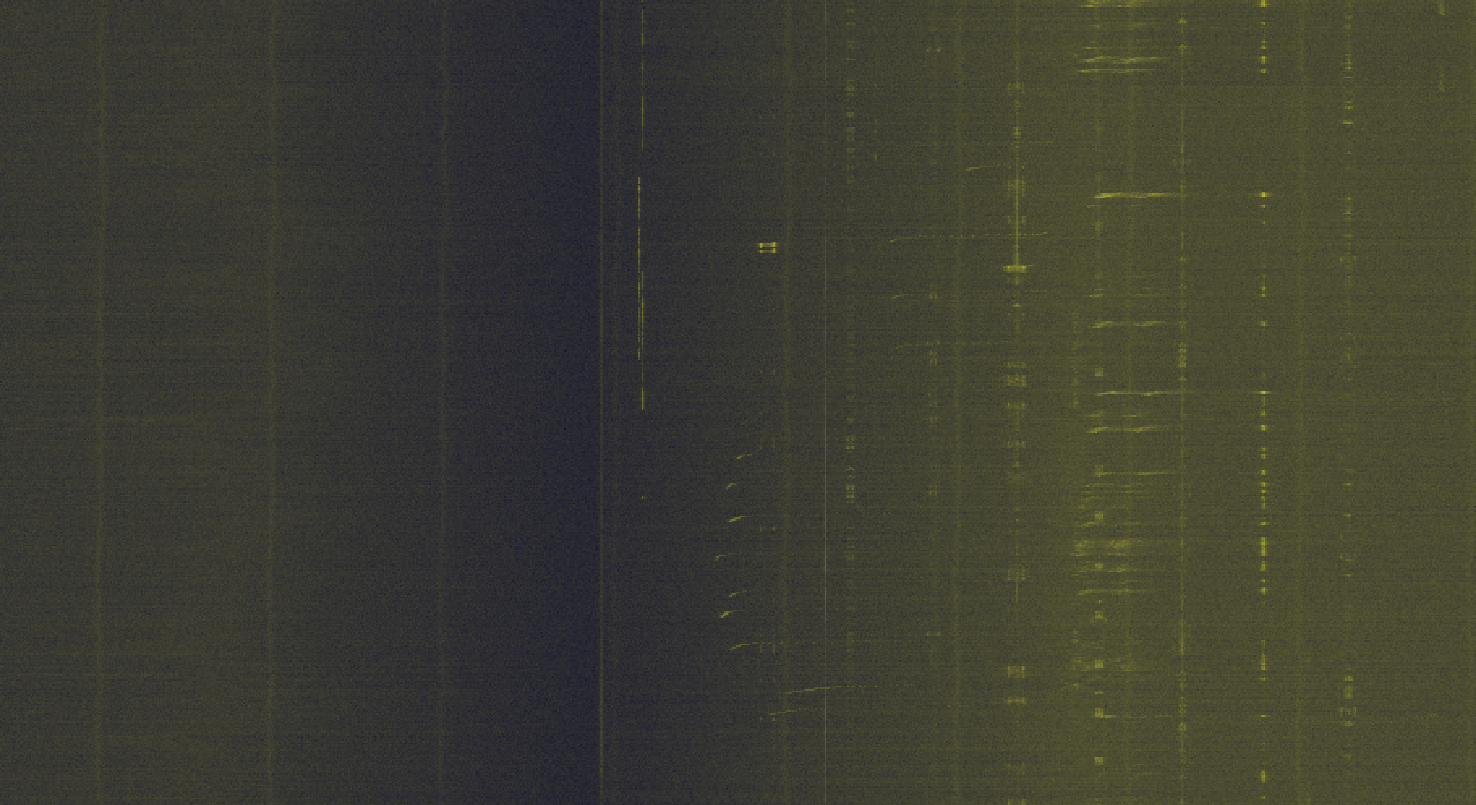
\includegraphics[width=5cm]{images/80}
		\caption{Spectrogram 1st August 2015}
		\label{fig:rtl_power_spectrogram_01} 
	\end{subfigure}
	\quad
	\begin{subfigure}[t]{5cm}
		\centering
		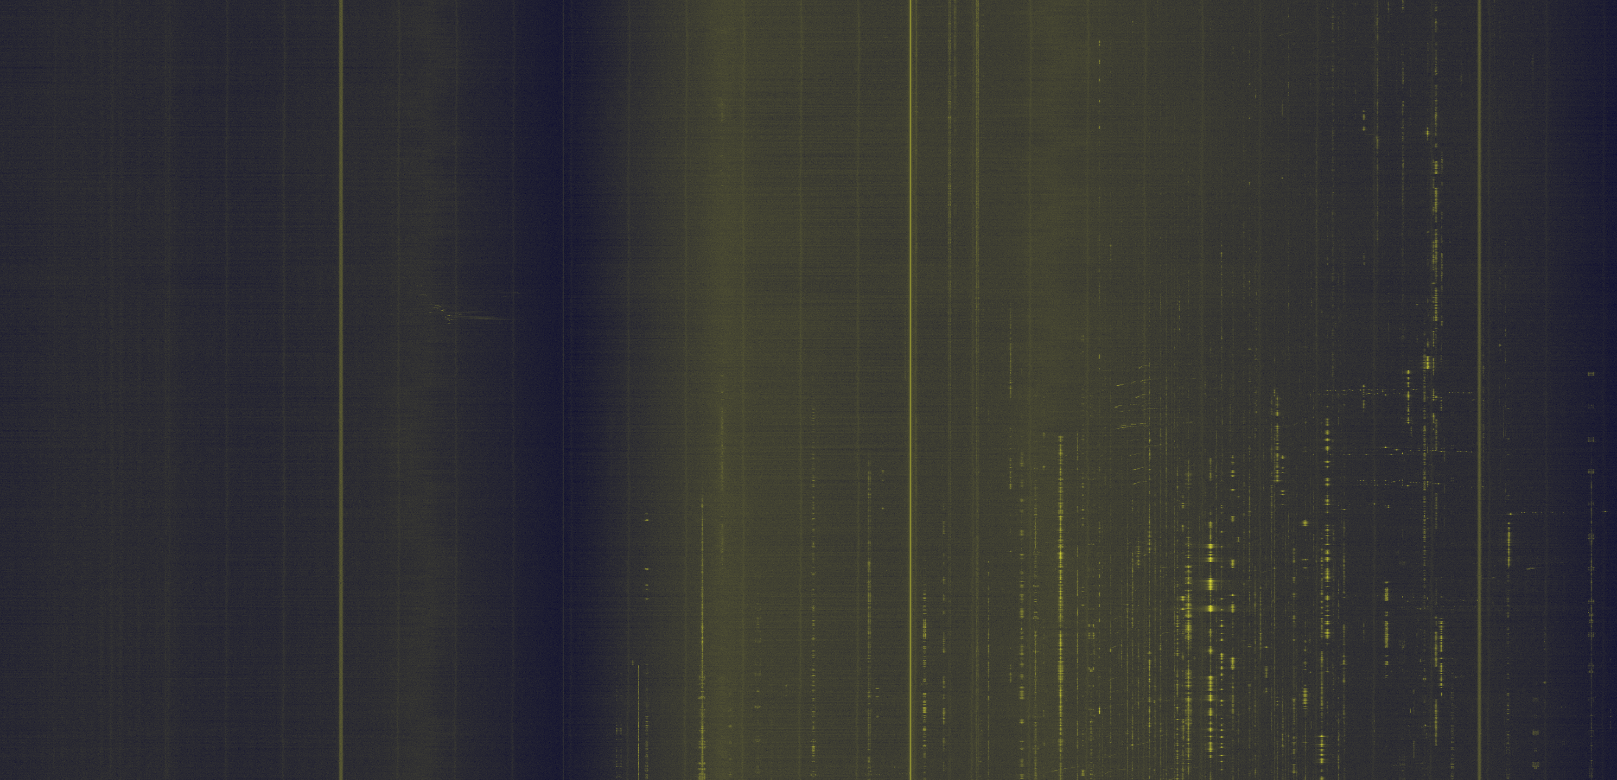
\includegraphics[width=5cm]{images/77}
		\caption{Spectrogram 28th July 2015}
		\label{fig:rtl_power_spectrogram_02} 
	\end{subfigure}
	\quad
	\begin{subfigure}[t]{5cm}
		\centering
		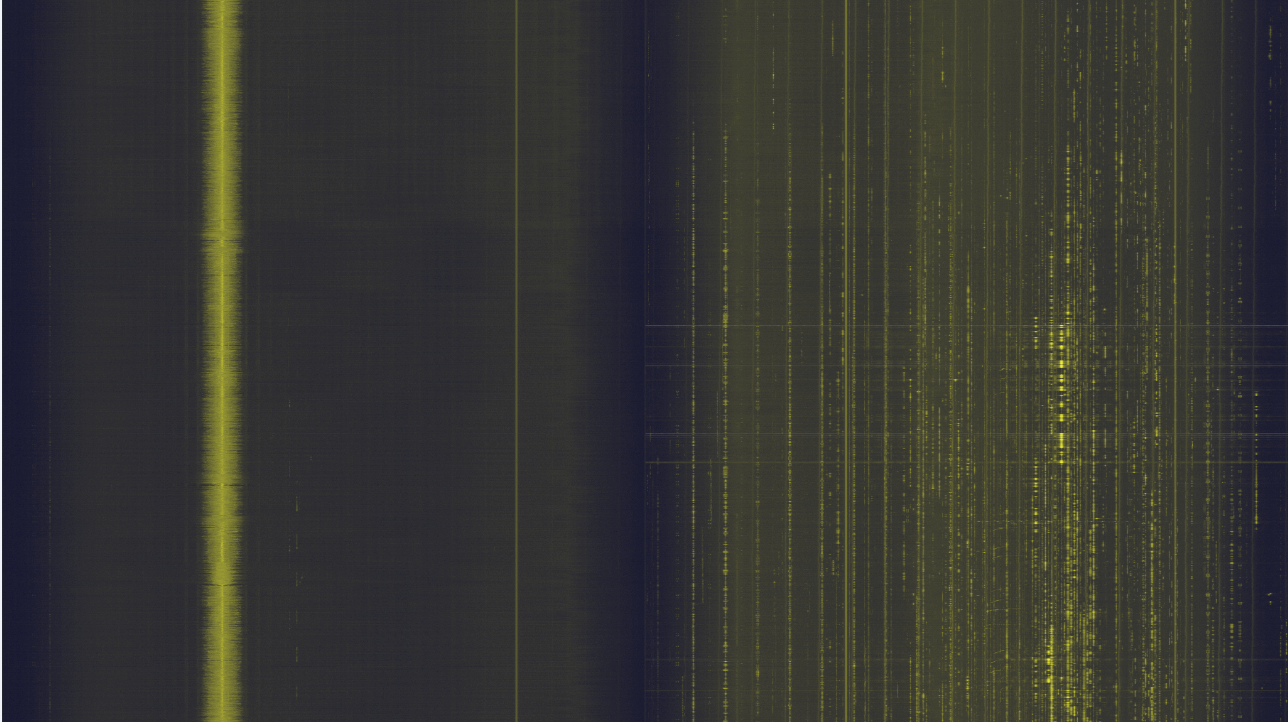
\includegraphics[width=5cm]{images/78}
		\caption{Spectrogram 17th July 2015}
		\label{fig:rtl_power_spectrogram_03} 
	\end{subfigure}
	\quad
	\begin{subfigure}[t]{5cm}
		\centering
		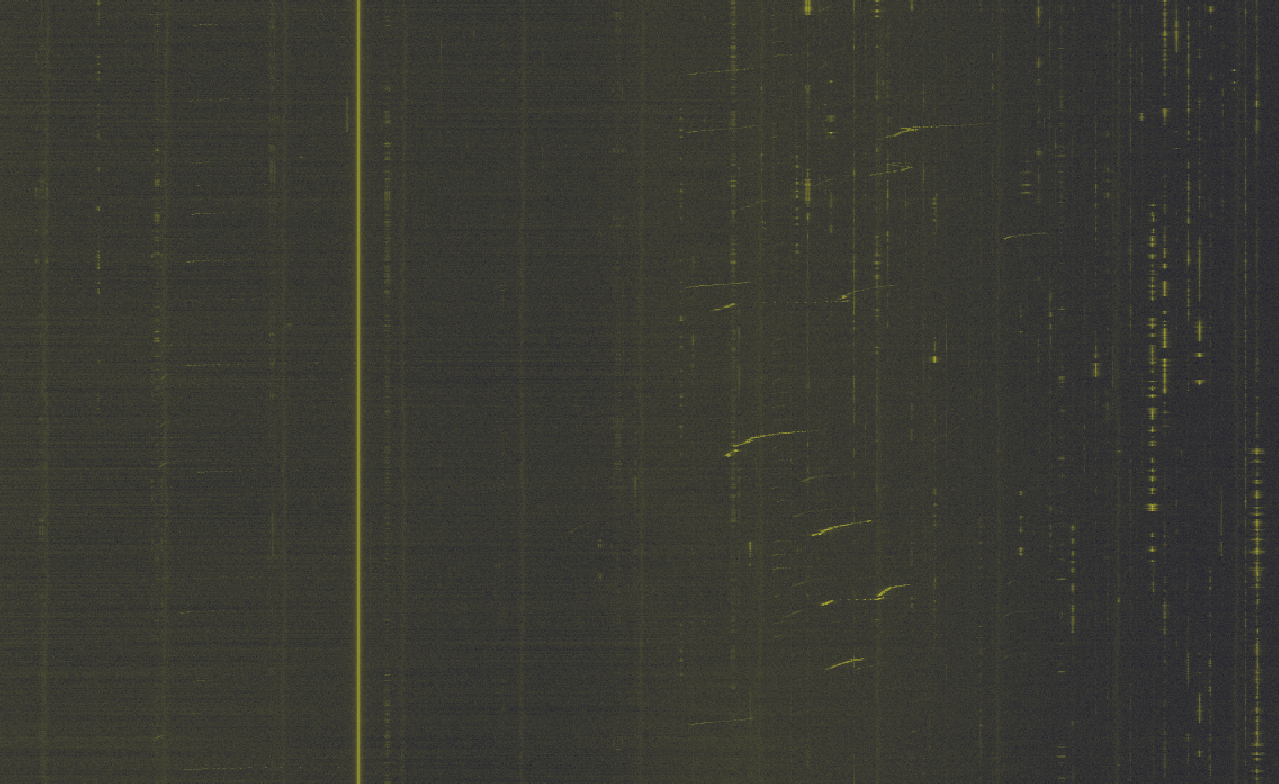
\includegraphics[width=5cm]{images/79}
		\caption{Spectrogram 14th July 2015}
		\label{fig:rtl_power_spectrogram_04} 
	\end{subfigure}
	\quad

	\caption{24MHz - 28MHz Spectrograms of rtl\_power data plotted using heatmap.py}
	\label{fig:rtl_power_spectrogram}
\end{figure}
%

%
\begin{figure}	
	\centering
	\begin{subfigure}[t]{8cm}
		\centering
		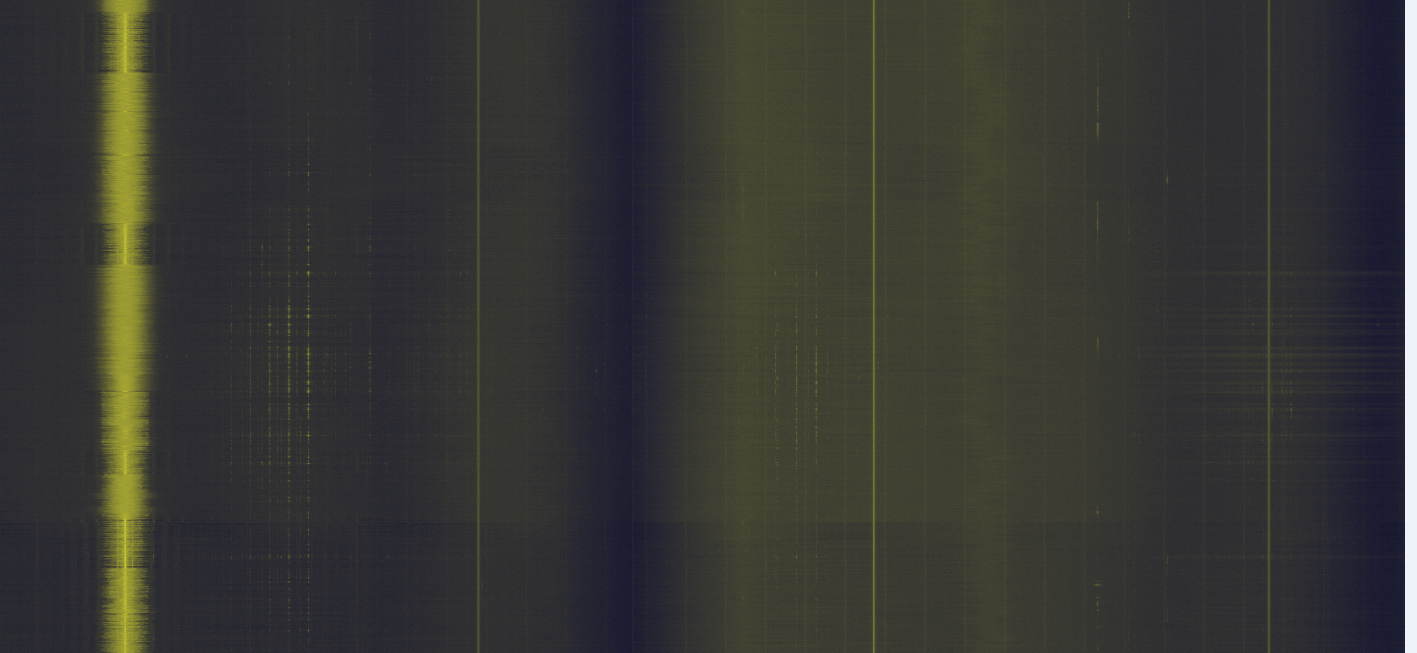
\includegraphics[width=8cm]{images/81}
		\caption{Spectrogram 10th July 2015}
		\label{fig:rtl_power_spectrogram_05} 
	\end{subfigure}
	\quad
	\begin{subfigure}[t]{8cm}
		\centering
		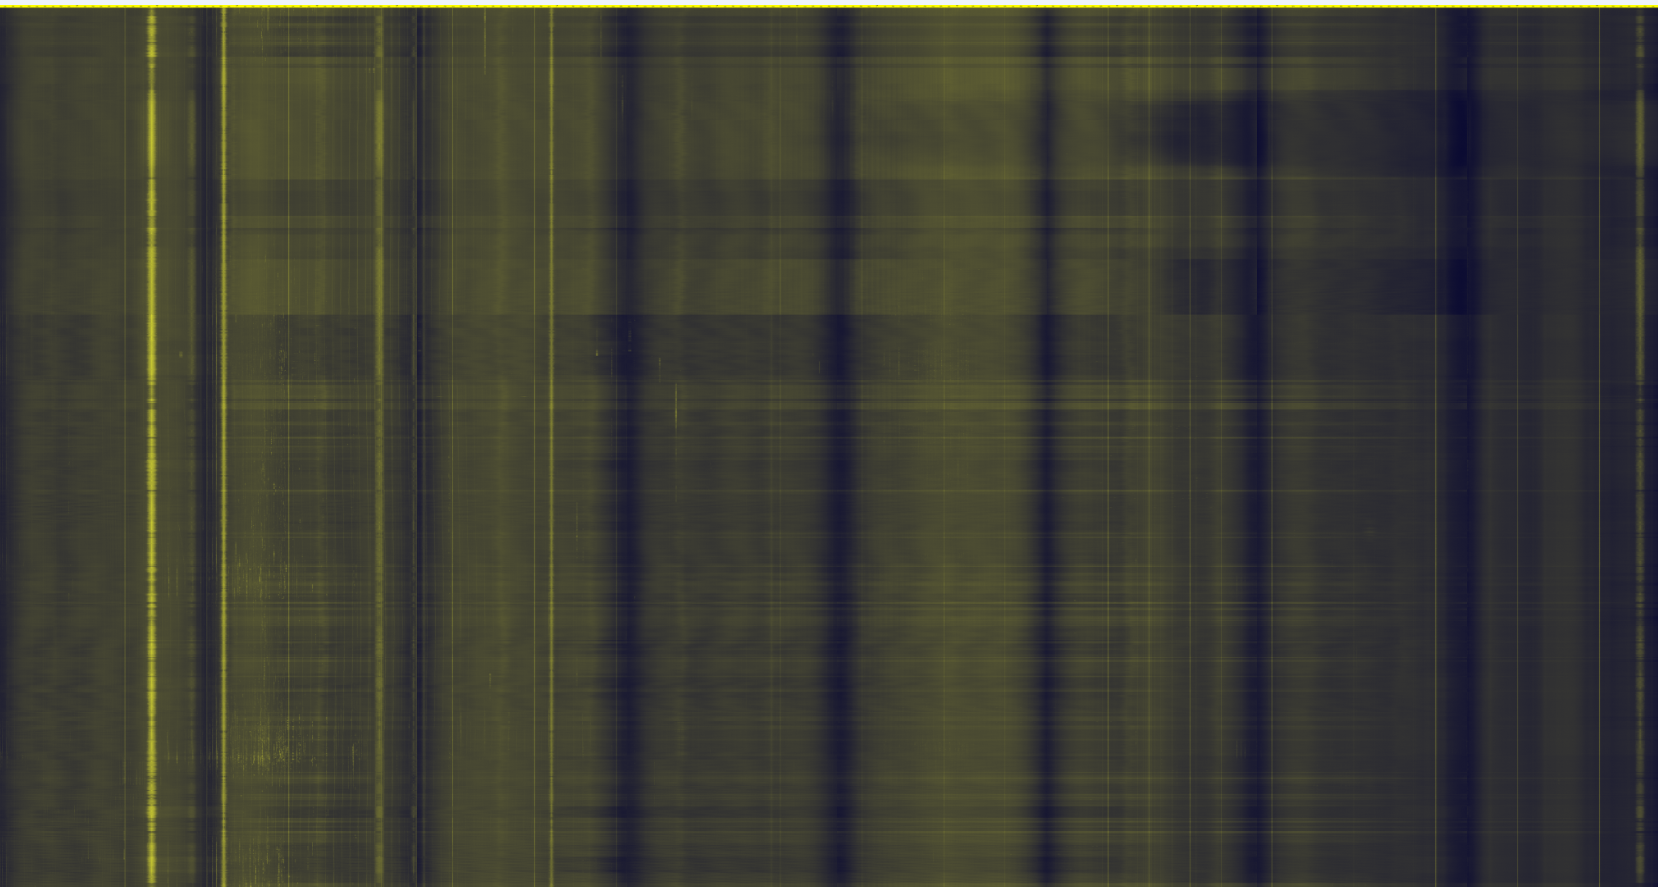
\includegraphics[width=8cm]{images/82}
		\caption{Spectrogram 25th June 2015}
		\label{fig:rtl_power_spectrogram_06} 
	\end{subfigure}
	\quad
	\begin{subfigure}[t]{8cm}
		\centering
		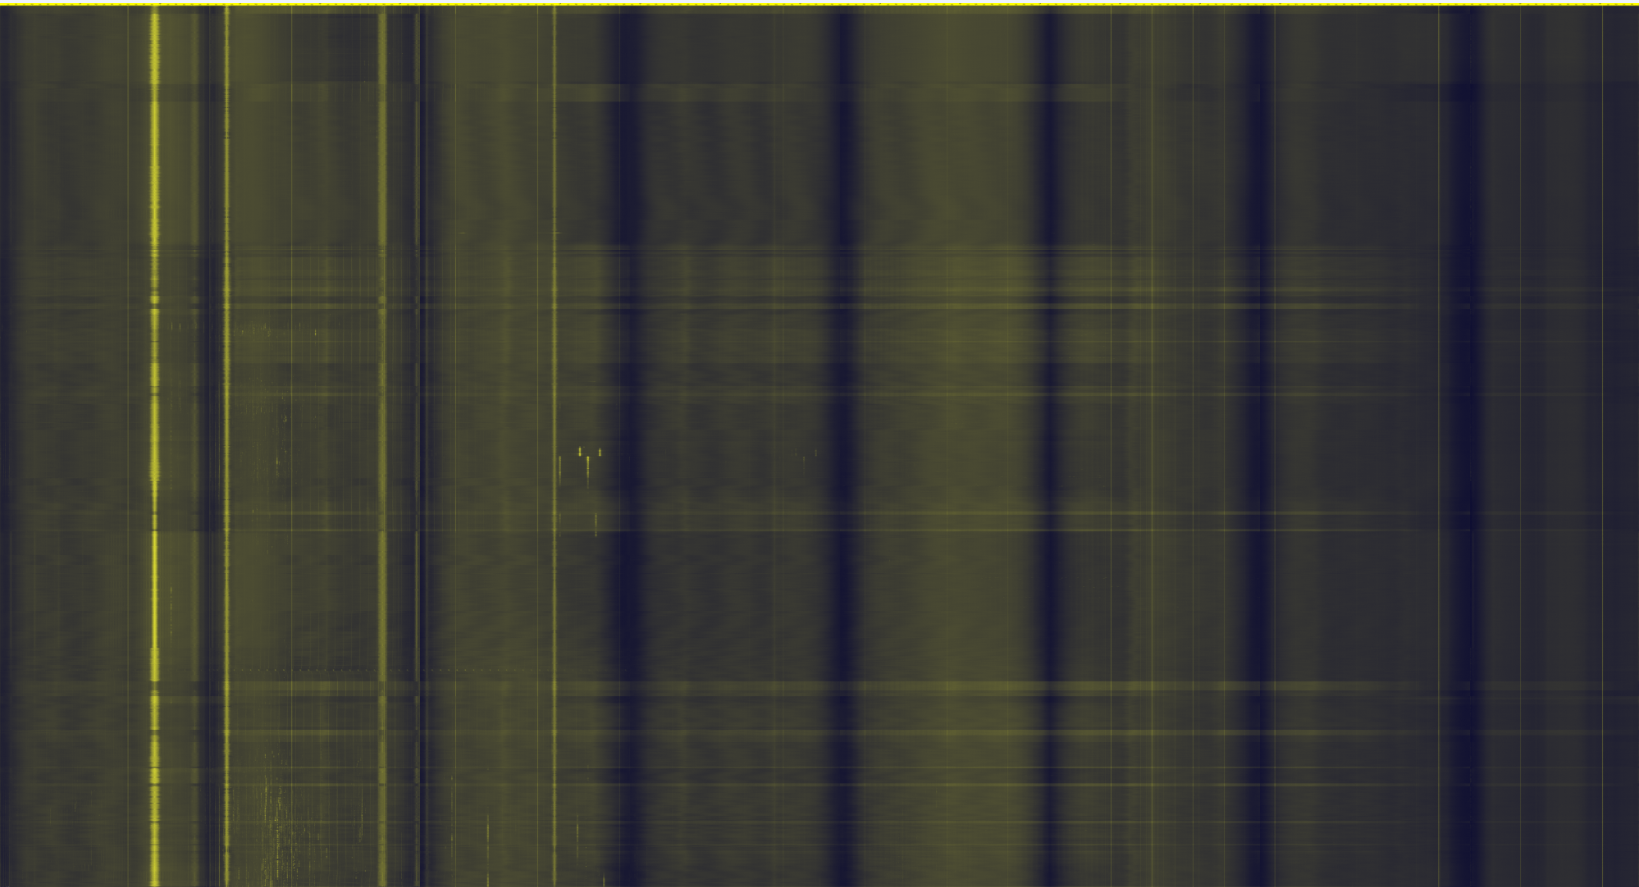
\includegraphics[width=8cm]{images/83}
		\caption{Spectrogram 24th June 2015}
		\label{fig:rtl_power_spectrogram_07} 
	\end{subfigure}
	\quad
	\begin{subfigure}[t]{8cm}
		\centering
		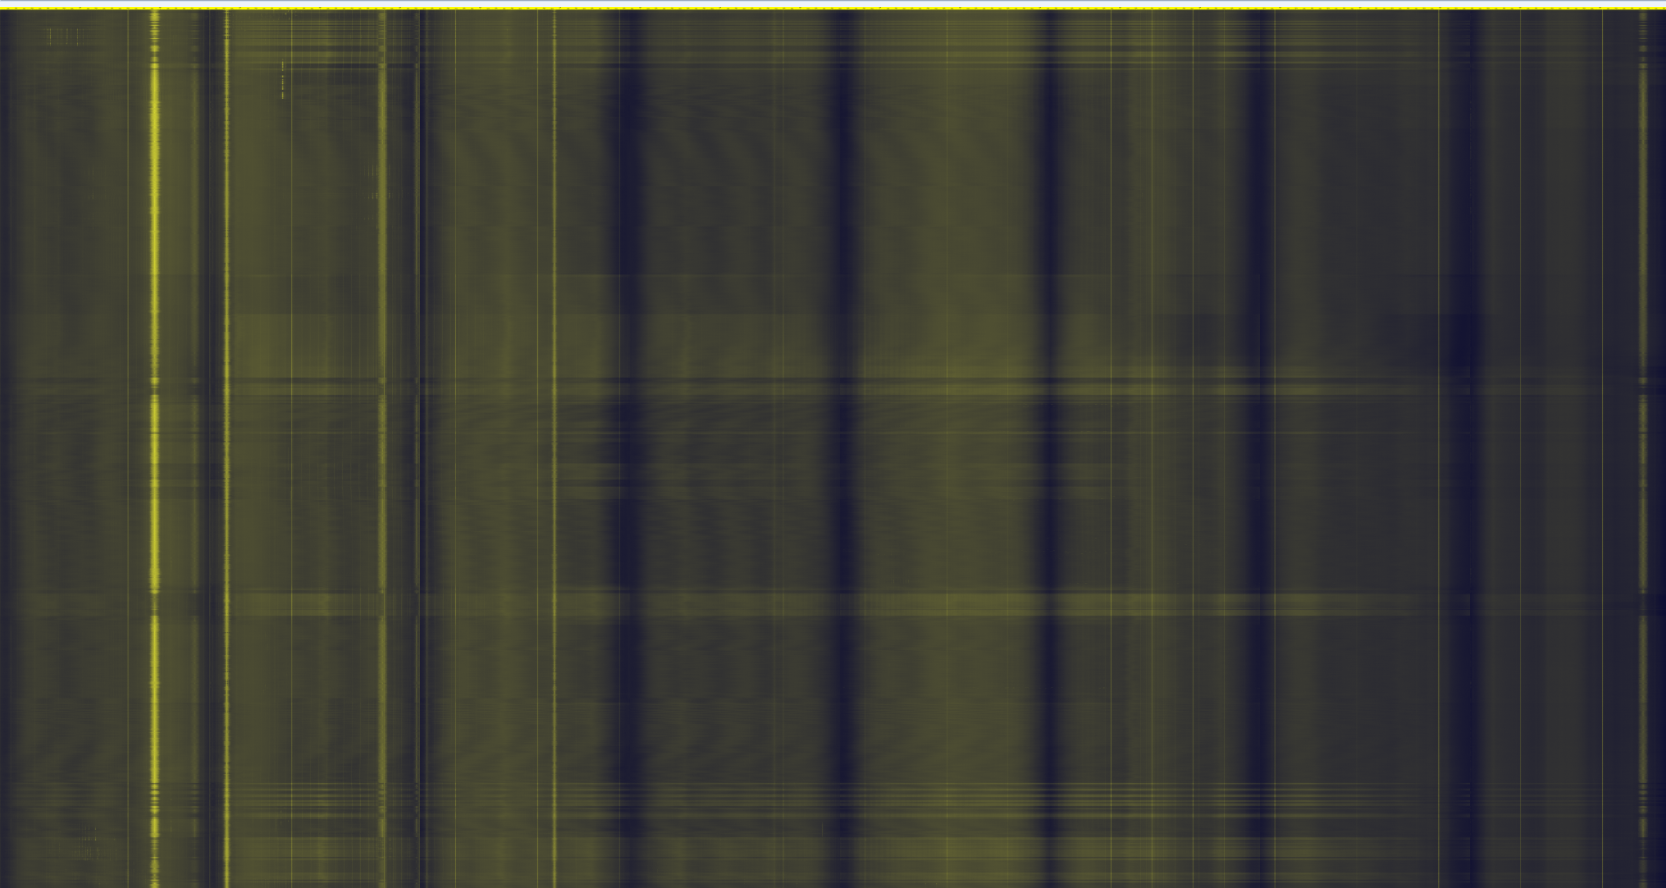
\includegraphics[width=8cm]{images/84}
		\caption{Spectrogram 23rd June 2015}
		\label{fig:rtl_power_spectrogram_08} 
	\end{subfigure}
	\quad
	\caption{24MHz - 40MHz Spectrograms of rtl\_power data plotted using heatmap.py}
	\label{fig:rtl_power_spectrogram_dam}
\end{figure}
%


\newpage
\section*{Implementing a HackRF Compatible Flow-Graph in GNURadio}
\addcontentsline{toc}{section}{Implementing a HackRF Compatible Flow-Graph in GNURadio}

As mentioned previously there is currently no existing tool which is capable of generating spectrogram plots using a HackRF transceiver from previously saved data. In order to rectify this, the methods of generating spectrograms was investigated. One method requires that the digital signal is broken up into chunks of the original bandwidth, and measured using a total power meter. It is not possible to measure the power at an individual frequency, a band of frequencies must be measured instead \citep{keen-15}.

Figures: \ref{fig:kuisma-iq-helix} and \ref{fig:signal_modulation} shows how a signal is stored digitally once sampled as an I/Q plot. Each data point stored contains the in phase component and the quadrature phase component. The equation shown in Figure: \ref{fig:power_formula} can be used in order to calculate the total noise power from such a I/Q digital sample \citep{nelson-15}.

%
\begin{figure}[here]
	\centering
	\begin{equation}
	Power = I^2 + Q^2
	\end{equation}
	\caption{Converting in-phase and quadrature-phase to power values}
	\label{fig:power_formula}
\end{figure}
%

The equation listed in Figure: \ref{fig:power_formula} has been implemented in within a GNURadio flow-graph and contains a software implementation of a total power radiometer \citep{nelson-15}. The functionality of a radiometer or total power meter provides the means to measure a chunk of bandwidth from a sample and produce a total noise power value which can then be plotted or used elsewhere within a larger GNURadio flow-graph.

%
\begin{figure}[!htb]
	\centering
	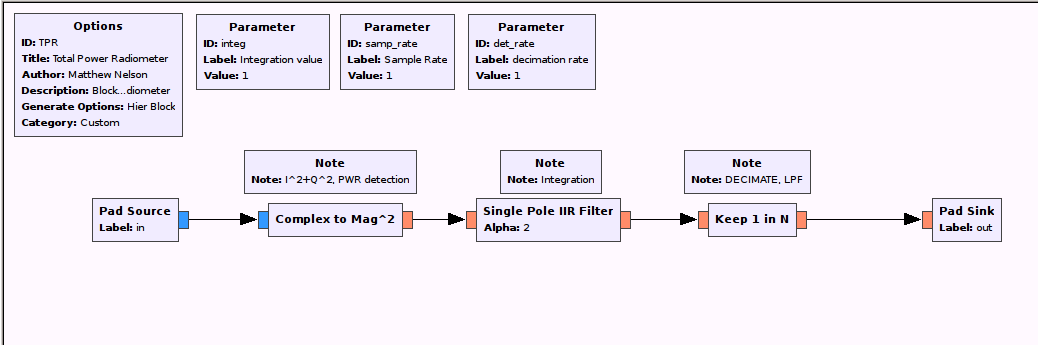
\includegraphics[width=8cm]{images/17}
	\caption{Total Power Meter Implemented in GNURadio \citep{nelson-15}}
	\label{fig:sdr_total_power_meter} 
\end{figure}
%

%
\begin{figure}[!htb]
	\centering
	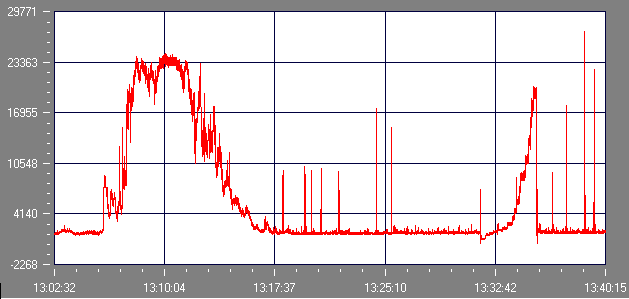
\includegraphics[width=8cm]{images/18}
	\caption{Radio Skypipe Software Power Plot \citep{rsp-15}}
	\label{fig:radio_skypipe_power_plot}
\end{figure}
%

\subsection*{Methodology}
The following methodology was followed during this experiment:

\begin{enumerate}
	\item Design a GNURadio flow-graph prototype to generate a set of test signals
	\item Design a GNURadio flow-graph prototype to which filters a signal using a bandpass filter
	\item Design a GNURadio flow-graph which incorporates the total power meter in order to produce a power plot
\end{enumerate}

The Figure: \ref{fig:radio_skypipe_power_plot} shows a voltage power graph generated using the Radio Skypipe software \citep{rsp-15}. Such a graph can be produced by measuring the power from a band of frequency and plotting the values against time. A prototype GNURadio flow-graph (Figure: \ref{fig:gnuradio_companion_flowgraph_01}) was designed which generates a test signal as seen in Figure: \ref{fig:gnuradio_companion_flowgraph_02}. This signal was then passed through a bandpass filter, which removes signals outside the permitted frequency range, the result of which can be seen in Figure: {\ref{fig:gnuradio_companion_flowgraph_03}}.

This flow-graph provided the means to isolate and measure the power for individual bands of frequency while ignoring frequencies outside this range. This flow-graph (Figure: \ref{fig:gnuradio_companion_flowgraph_05}) was then upgraded to incorporate the total power meter as seen in Figure: \ref{fig:gnuradio_companion_flowgraph_04}. It is possible to capture live power data within a frequency band directly from a osmocom source such as the HackRF, or alternatively from previously recorded data. 

A power graph was generated from I/Q data collected during the 20th March 2015 for the solar eclipse radio propagation experiment. The plot shows the signal power (V) rise as the eclipse reaches max totality and can be seen in Figure: \ref{fig:gnuradio_companion_flowgraph_06}, which compliments the previously generated signal power (dB) plot shown in Figure: \ref{fig:signal_power_v_time_radio_propagation}.

Radiometers can be used to produce signal intensity plots and thereby allow the detection of very faint natural radio emissions such as the Jovian \gls{DAM} emissions, cosmic microwave background and other discrete astronomical sources such as galaxies \citep{nrao-10}. In order to make use of a radiometer attached to the telescope for radio astronomical applications it must first be calibrated. \cite{nelson-15} suggested the use of 3 sources with known temperatures as demonstrated in Figure: \ref{fig:calibrated_radiometer} in order to calibrate the radiometer.

\citet{nelson-15} collected measurements while the radiometer was immersed in ice water. Next the load was placed in the liquid nitrogen bath and finally in boiling hot water. A linear algebra model was developed in order to convert the total power readings to Kelvin values thereby calibrating the data. Figure: \ref{fig:calibrated_radiometer} shows the calibrated values \citep{nelson-15}.

%
\begin{figure}	
	\centering
	\begin{subfigure}[t]{8cm}
		\centering
		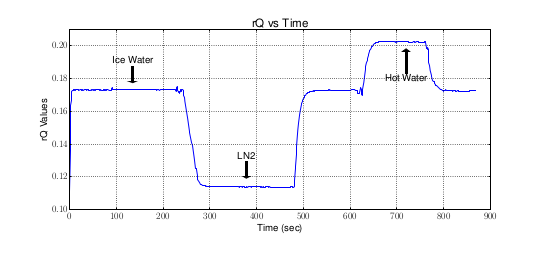
\includegraphics[width=8cm]{images/89}
		\caption{Graph of uncalibrated noise temperature \citep{nelson-15}}
		\label{fig:uncalibrated_radiometer} 
	\end{subfigure}
	\quad
	\begin{subfigure}[t]{8cm}
		\centering
		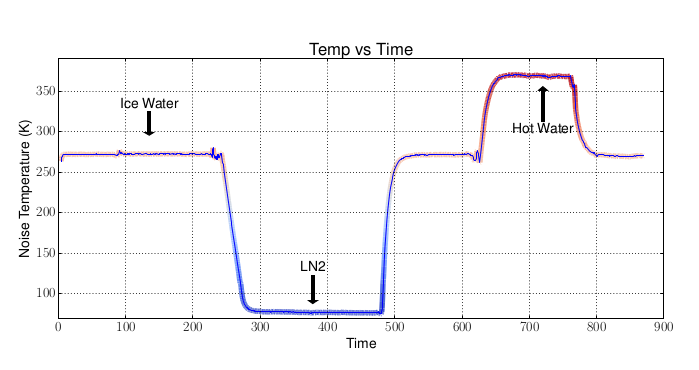
\includegraphics[width=8cm]{images/87}
		\caption{Graph of calibrated noise temperature \citep{nelson-15}}
		\label{fig:calibrated_radiometer}
	\end{subfigure}
	\caption{Calibration of the SDR Radiometer}
	\label{fig:sdr_radiometer_calibration}
\end{figure}
%


%
\begin{figure}	
	\centering
	\begin{subfigure}[t]{5cm}
		\centering
		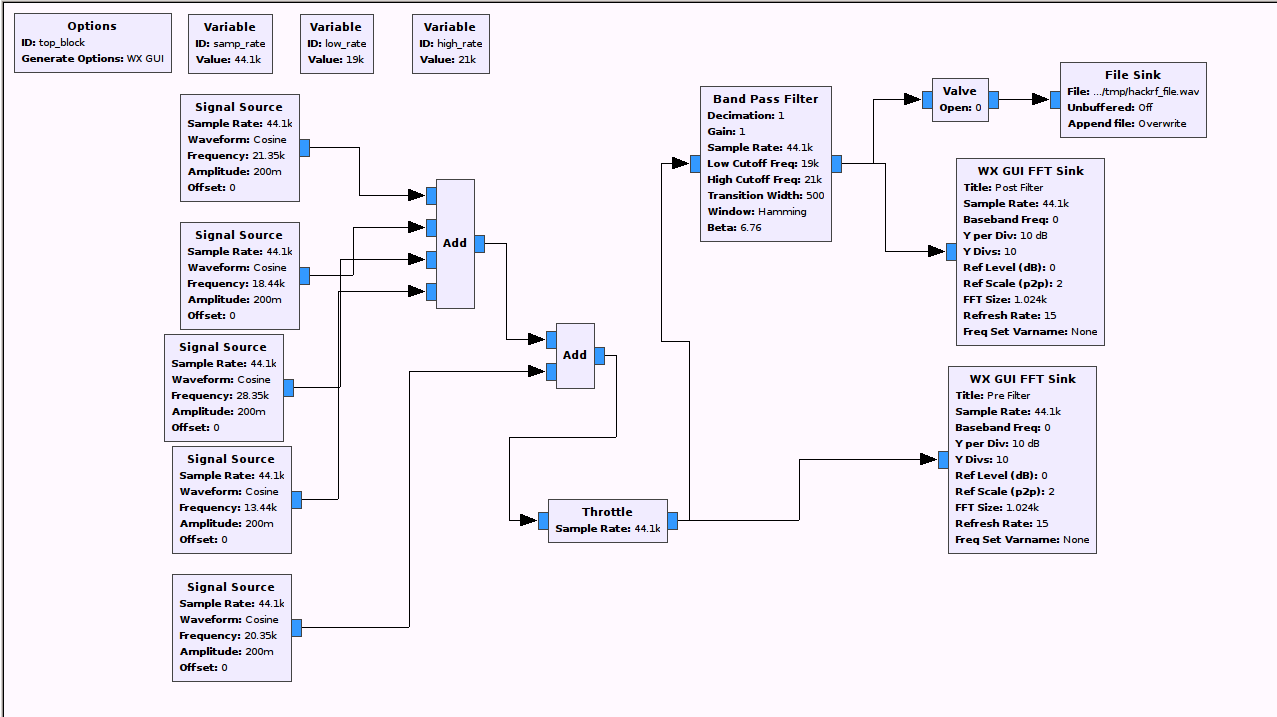
\includegraphics[width=5cm]{images/21}
		\caption{Prototype flow-graph to generate test signals and filter frequencies}
		\label{fig:gnuradio_companion_flowgraph_01} 
	\end{subfigure}
	\quad
	\begin{subfigure}[t]{5cm}
		\centering
		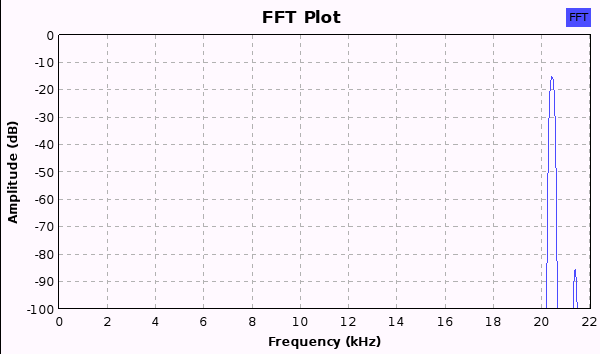
\includegraphics[width=5cm]{images/22}
		\caption{Test signal FFT plot}
		\label{fig:gnuradio_companion_flowgraph_02} 
	\end{subfigure}
	\quad
	\begin{subfigure}[t]{5cm}
		\centering
		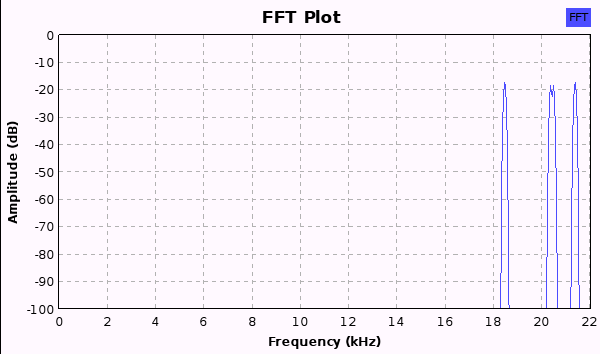
\includegraphics[width=5cm]{images/23}
		\caption{Filtered test signal FFT plot}
		\label{fig:gnuradio_companion_flowgraph_03} 
	\end{subfigure}
	\quad
	\begin{subfigure}[t]{5cm}
		\centering
		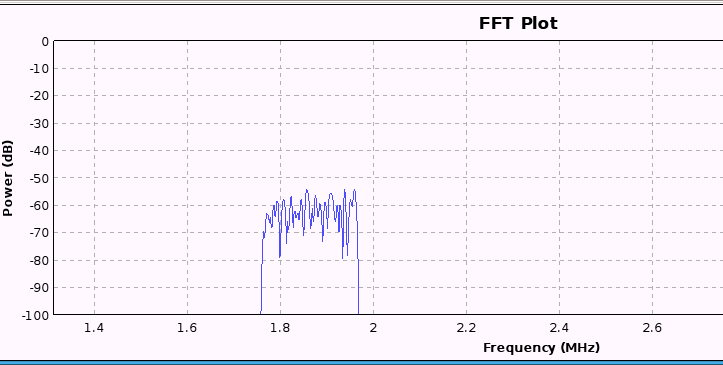
\includegraphics[width=5cm]{images/76}
		\caption{Solar eclipse signal filtered to isolate radio station}
		\label{fig:gnuradio_companion_flowgraph_04} 
	\end{subfigure}
	\quad
	%
	\begin{subfigure}[t]{8cm}
		\centering
		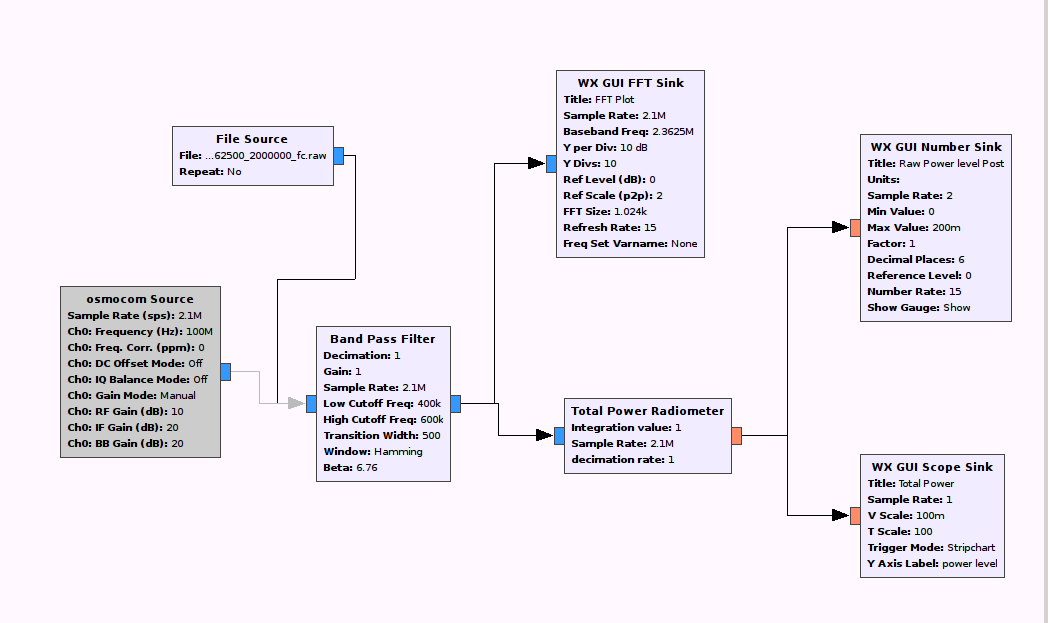
\includegraphics[width=8cm]{images/85}
		\caption{Flow-graph incorporating filtering and total power meter capability}
		\label{fig:gnuradio_companion_flowgraph_05}
	\end{subfigure}
	%
	\quad
	\begin{subfigure}[t]{8cm}
		\centering
		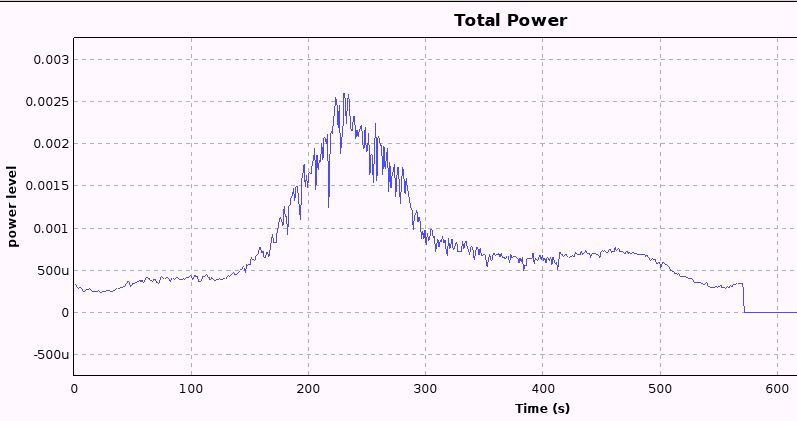
\includegraphics[width=8cm]{images/75}
		\caption{Total power (V) plotted against time for radio station recorded during solar eclipse}
		\label{fig:gnuradio_companion_flowgraph_06} 
	\end{subfigure}
	\caption{GNURadio flow-graphs to generate total power plots from saved data}
	\label{fig:gnuradio_companion_flowgraph}
\end{figure}
%
